\title{Project Ingenieurswetenschappen \\ Het elektronisch ontwerp van de e-VUBOX speaker}
\author{Vrije Universiteit Brussel}
\date{Versie 08.2015}

\documentclass[11pt]{article}
	%\usepackage[a4paper]{geometry}
	%\usepackage[utf8x]{inpudetenc}
	\usepackage[T1]{fontenc}
	\usepackage[dutch]{babel}
	\usepackage{amsmath}
	%%% FIGURES %%%
	\usepackage[pdftex]{graphicx}
	\usepackage{caption,subcaption}
	\usepackage{hyperref}
	\graphicspath{ {./figs/} }

\begin{document}
\maketitle
\begin{figure}[htbp]
	\centering
	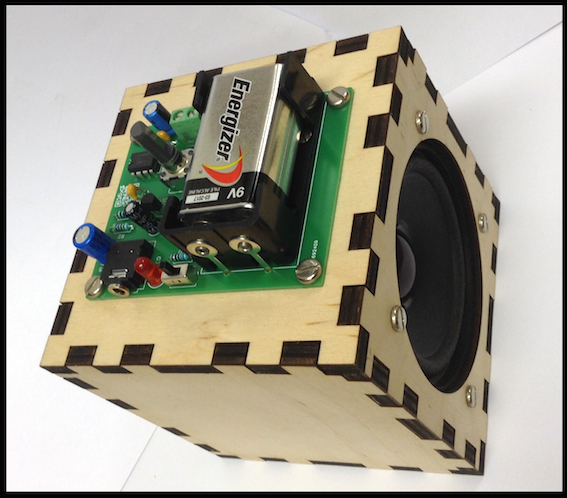
\includegraphics[width=0.8\textwidth]{foto.jpg}
	\caption{De prachtige e-VUBOX.}
	\label{fig:foto}
\end{figure}

\clearpage
\tableofcontents
\clearpage

\section{Doelstelling}
Elektronische uitvindingen maken deel uit van de grote revoluties van deze eeuw. Van de simpele rekenmachine tot de meest geavanceerde gaming-PC, GPS-satellieten, zelfrijdende auto's, implantaten die het zicht van blinde pati�nten herstellen, robots die duizenden objecten per seconde herkennen en een zinnige gesprek met mensen kunnen houden... Die verbluffende uitvindingen worden dagelijks gemaakt en gebruikt.

Al die fascinerende ontwikkelingen kunnen het gevoel geven dat je graag eens zelf elektronische netwerken zou willen bouwen, als je maar wist hoe die miraculeuse elektronica in mekaar zat. Goed nieuws, dit is het net doel van dit project: we gaan de mysteries van de elektronica ontfutselen door \textbf{een audio-versterker te bouwen}. Je zal snel zien dat elektronische circuits niet (helemaal) magisch zijn en daarenboven nog goedkoop zijn om zelf te maken!

%We gaan beginnen met een inleiding in de elektronica. Daar gaan we kennismaken met basisregels die nodig zijn om componenten en schakelingen te begrijpen en zelf te ontwerpen. Daarna stappen we over naar naar complexere onderdelen en gaan we onze eigen versterker bouwen.

%Waarom zou je elektronica willen leren? Wel, elektronica kan interessant zijn om te bestuderen omdat veel leuke en/of nuttige objecten mogelijk zijn dankzij de elektronica. Alledaagse objecten zoals een GSM of een computer bevatten natuurlijk veel elektronica, maar ook in het ziekenhuis kan je ook toestellen vinden die dagelijks levens redden, zoals een MRI-scanner of een elektrocardiogram. Zelfs de wereld van entertainement zit boordevol elektronische netwerken: in cameras, schermen, spelconsoles, virtuele werkelijkheid, enz.. Veel geavanceerde technologi�en zoals het internet, zelfrijdende autos, de automatische piloot in vliegtuigen en andere robots met artifici�le intelligentie zouden ook niet mogelijk zijn zonder o.a. ingenieurs in de elektronica.

% Indien je dit al hebt gezien, mag je het deel ``Elektronica: componenten en schakelingen'' snel overlopen en onmiddelijk beginnen met het hoofdstuk \ref{sec:bouwstenen} op pagina \pageref{sec:bouwstenen}. 
Laten we beginnen met een overzicht van de wetten en vuistregels van de elektronica. Als je ze al heb gezien, mag je onmiddelijk beginnen met hoofdstuk \ref{sec:bouwstenen}.
\section{Elektronica: componenten en netwerken}

De Van Dale definie�rt elektronica als "de wetenschap die studie maakt van de geleiding van elektronen en van de mogelijke toepassingen daarvan".
Dankzij het schakelen van elektronische componenten in een elektronisch netwerk, kunnen we de elektronen temmen zodat ze ons helpen om specifieke taken uit te voeren zoals het bewegen van een arm van een robot of het versterken van muziek.

% Dit doen we door netwerken van elektronische componenten te bouwen. Elektronische componenten zijn eenvoudige bouwstenen waarmee we complexe netwerken kunnen bouwen op zo een manier dat die specifieke taken uitvoeren: het ontvangen en versturen van de meest belangrijke berichtjes via Messenger, het afbeelden van een foto op een scherm en vele andere toepassingen die je elke dag tegenkomt. %Je hebt waarschijnlijk een object vol elektronica in jouw broekzak op dit ogenblik!

De schematische voorstelling van elektronische componenten en een netwerk zijn te vinden in Figuur \ref{fig:component_en_schakeling}. Met pijltjes zijn de twee grootheden aangeduid die in de elektronica zeer belangrijk zijn :

\begin{enumerate}
	\item de \textbf{spanning} (ook voltage of potentiaal genoemd) gemeten in volt [V], vaak aangeduid met de letter $V$ of $U$. Dit stelt het verschil voor in potenti�le elektrische energie \textbf{tussen twee punten} \footnote{Je kent al een maat voor het verschil in potienti�le gravitationele energie: de hoogte in meter. Zoals een bal valt van hoog naar laag, gaat een positieve lading lopen van een hoge spanning naar een lage spanning.}. Vaak wordt er gesproken van de spanning \textbf{op} een punt, dit moet je begrijpen als het spanningsverschil \textbf{tussen} dat punt en de grond, een bijzonder punt die je binnenkort ook zal kennen .%De spanning is altijd een \textbf{verschil}: de spanning  $V$ over de componenten in figuur \ref{subfig:componenten} is bijvoorbeeld $V = V_2-V_1$. 

	\item de \textbf{stroom} gemeten in amp�re [A], vaak aangeduid met de letter $I$. Dit stelt de verplaatsing voor van een hoeveelheid ladingen (hier elektronen) door de component per tijdseenheid.
\end{enumerate}

Stromen en spanning kunnen constant over de tijd zijn, we spreken dan van DC (Direct Current). Als ze veranderen met de tijd, spreken we van AC (Alternating Current) en  kunnen ze beschreven worden door wiskundige functies zoals bijvoorbeeld:
\begin{align}
     I(t) = 0.1 \text{A} \cdot sin(t) \\
     V(t) = 4 \text{V} \cdot e^{-\frac{t}{10 s}}
 \end{align} 
 waar $t$ de tijd is in seconden.

\begin{figure}[hbtp]
	\centering
	\begin{subfigure}[b]{0.45\linewidth}
		\centering
		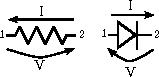
\includegraphics[width=0.8\linewidth]{componenten}
		\caption{Elektronische componenten: een weerstand links en een diode rechts. Men spreekt van de spanning $V$ \textbf{over} de pinnen (1 en 2), en de stroom $I$ \textbf{door} de component. Let op: de zin van de pijlen heeft belang!}
		\label{subfig:componenten}
	\end{subfigure}
	~
	\begin{subfigure}[b]{0.45\linewidth}
		\centering
		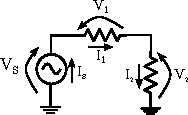
\includegraphics[width=0.8\linewidth]{weerstandsdeler}
		\caption{Elektronisch netwerk: een schakeling van componenten. Er is \textbf{over} elk component een spanningsval , en \textbf{door} elk component een stroom.}
		\label{subfig:netwerk}
	\end{subfigure}
	\caption{Componenten en een schakeling. }
	\label{fig:component_en_schakeling}
\end{figure}

Heel de magie van de elektronica zit in de componenten die voldoen aan zekere I-V (stroom-spanning) relaties die worden bepaald dankzij hun fysica. Bijvoorbeeld: In de weerstand is de stroom evenredig met de spanning en in de diode vloeit stroom maar in ��n richting. We gaan interessante componenten leren kennen en gebruiken, en gaan onmidellijk beginnen met de gewoonste (en meest gebruikte) component: de weerstand.

 %Elke component in de elektronica voldoet aan fysische wetten die zijn stroom en de spanning bepalen. Laten we kennismaken met die fysische wetten, en daarna we gaan onmiddellijk ons eerste netwerk oplossen. We bekijken twee basiselementen van de elektronica: de weerstand en de spanningsbron.

\subsection{De weerstand}

 Een weerstand (figuur \ref{subfig:componenten}) is een geleider die voldoet aan de \textbf{wet van Ohm} (stroom en spanning zijn evenredig): 
\begin{align}
	V &= R \cdot I
\end{align} 
$R$ is een eigenschap van de weerstand die men ook elektrische weerstand noemt, met eenheid Ohm\footnote{Georg Simon Ohm (1787 - 1854) was een Duits wiskundige en natuurkundige, ontdekker van de wet van Ohm in 1827.} [$\Omega$]. $V$ is de spanning over de weerstand en $I$ de stroom door de weerstand.

Een manier om weerstanden te bezien is als belemmers van stroom. Een grote weerstand heeft een hoge spanningsval nodig om veel stroom te verplaatsen. 

%Zo dadelijk volgt een voorbeeld, we gaan eerst zien wat weerstanden in serie en in parallel zijn, en kennismaken met de spanningsbron.

\subsubsection{Serie en parallel}
\label{sssec:serie_en_parallel}
Soms kan je twee weerstanden door een weerstand vervangen als ze speciaal samenzitten en dat kan het ontwerpen vergemakkelijken. Dit kan in twee gevallen (zie figuur \ref{fig:serie_en_parallel}):

\begin{itemize}
	\item twee weerstanden zijn \textbf{in serie}: ze hebben ��n gemeenschappelijke pin, en dezelfde stroom vloeit door de twee weerstanden, dan is de vervangingsweerstand :
	\begin{align}
		R_{v} = R_1 +R_2.
	\end{align}
	Door weerstanden in serie te plaatsen, krijg je dus een grotere weerstand.

	\item twee weerstanden staan \textbf{parallel}: de twee weerstanden hebben beide pinnen gemeenschappelijk, dus de spanning over de twee is dezelfde. Dan geldt voor de vervangingsweerstand 
	\begin{align}
		\frac{1}{R_{v}}= \frac{1}{R_{1}} + \frac{1}{R_{2}} 
	\end{align}
	Door weerstanden in parallel te plaatsen, krijg je een kleinere weerstand.
\end{itemize}

\begin{figure}[hbtp]
	\centering
	\begin{subfigure}[b]{0.45\linewidth}
		\centering
		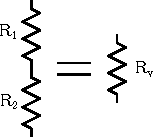
\includegraphics[width=0.5\linewidth]{serie}
		\caption{Weerstanden in serie.}
		\label{subfig:serie}
	\end{subfigure}
	~
	\begin{subfigure}[b]{0.45\linewidth}
		\centering
		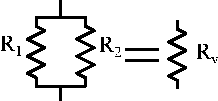
\includegraphics[width=0.8\linewidth]{parallel}
		\caption{Weerstanden in parallel.}
		\label{subfig:parallel}
	\end{subfigure}
	\caption{Serie en parallel.}
	\label{fig:serie_en_parallel}
\end{figure}

\subsection{De spanningsbron}

\begin{figure}[hbtp]
	\centering
	\begin{subfigure}[b]{0.2\linewidth}
		\centering
		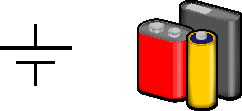
\includegraphics[width=0.4\linewidth]{vc}
		\caption{Constante spanningbron.}
	\end{subfigure}
	~
	\begin{subfigure}[b]{0.2\linewidth}
		\centering
		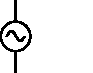
\includegraphics[width=0.4\linewidth]{vt}
		\caption{Vari�rende spanningsbron.}
	\end{subfigure}
	\caption{Spanningsbronnen.}
	\label{fig:vbron}
\end{figure}
 Een perfecte spanningsbron is een simpel elektronisch component met twee pinnen die gehoorzaamt aan een eenvoudige wet: de spanningsbron legt de spanning over zijn pinnen op, onafhankelijk van de rest van het netwerk. In werkelijkheid kan een spanningsbron maar een beperkte stroom leveren en gedraagt zich dan als een perfecte spanningsbron met een kleine weerstand in serie. Een 9V-batterij is een voorbeeld van een spanningsbron, die de spanning over zijn pinnen vastlegt op constant $9~V$. Een spanningsbron kan een constante spanning opleggen, maar niets verbiedt dat de spanning met de tijd verandert. Beide type bronnen hebben hun eigen schematische voorstelling die je kan vinden in figuur \ref{fig:vbron}.

\subsection{Mini-netwerk}
We gaan binnenkort wetten ontdekken van nog meer componenten, maar met onze voorlopige kennis kunnen we al volgend netwerk oplossen!
\paragraph*{Voorbeeld:} 
\begin{figure}[h!]
	\centering
	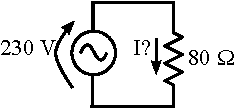
\includegraphics[width=0.25\textwidth]{vbweerstand.pdf}
	\caption{Voorbeeldnetwerkje.}
	\label{fig:vbweerstand}
\end{figure}

Een spanningbron legt en spanning op van $50~V$ over een weerstand van $200~\Omega$. Men kan de stroom door de weerstand berekenen op de volgende manier:

\begin{align}
	\text{(Wet van Ohm)}~V = R\cdot I \Leftrightarrow I = \frac{V}{R} \Leftrightarrow I = \frac{50~V}{200~\Omega}= 0,25~A
\end{align}

\paragraph*{Doe-het-zelf:} Wat is de waarde $R$ van een weerstand waarover een spanning van $V = 25~V$ is en waardoor een stroom van $I = 0.1~A$ loopt?
\\.\dotfill \\.\dotfill \\.\dotfill \\.\dotfill \\.\dotfill \\.\dotfill 

Elektronica is meer dan een spanningsbron en een weerstand, dus laten we maar een zien hoe grotere netwerken zich gedragen.

\subsection{Netwerken}

Een netwerk is een aaneenschakeling van componenten, die schematisch wordt voorgesteld zoals in figuur \ref{subfig:netwerk}. Er zijn maar twee regels die gelden voor elektrische/elektronische netwerken: de wetten van Kirchhoff\footnote{Gustav Robert Kirchhoff (1824 - 1887) was een Duits natuurkundige. Kirchhoff formuleerde zijn spanningswet en zijn stroomwet in 1845, toen hij nog een student was. Slimme kerel!}. Samen met de fysische wetten van de componenten kan je dan alle netwerken van de wereld oplossen. Een netwerk oplossen wilt zeggen dat je alle stromen en spanningen bepaalt in dat netwerk.

\paragraph*{De stroomwet van Kirchhoff:} in elk knooppunt in een elektrische kring is de som van de stromen die in dat punt samenkomen gelijk aan de som van de stromen die vanuit dat punt vertrekken. Dit is voor elk knooppunt geldig, onafhankelijk van de componenten die op de takken zijn. 
\paragraph*{De spanningswet van Kirchhoff:} de som van de elektrische potentiaalverschillen (rekening houdend met de richting) in elke gesloten lus in een kring is gelijk aan nul. 

\begin{figure}[htbp!]
	\centering
	\begin{subfigure}[b]{0.45\linewidth}
		\centering
		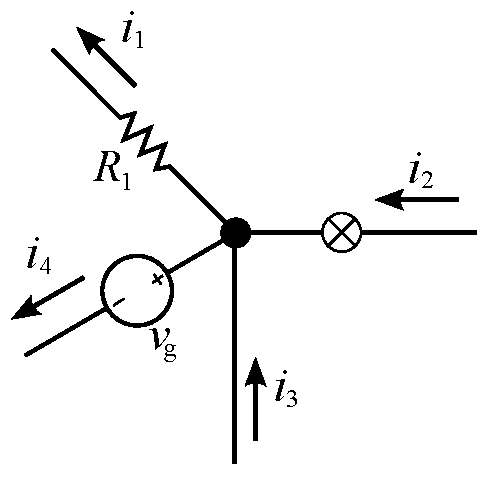
\includegraphics[width=0.8\textwidth]{kcl.pdf}
		\caption{In dit knooppunt is de stroomwet van Kirchhoff : $i_1 + i_4 = i_2+i_3$}
		\label{subfig:kcl}
	\end{subfigure}
	~
	\begin{subfigure}[b]{0.45\linewidth}
		\centering
		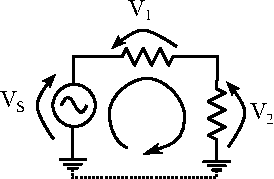
\includegraphics[width=0.9\textwidth]{kvl.pdf}
		\caption{In deze lus is is de spanningswet van Kirchhoff : $ + V_S - V_1 - V_2 = 0$}
		\label{subfig:kvl}
	\end{subfigure}
\caption{De wetten van Kirchhoff}
\label{fig:kirchoff}
\end{figure}

\paragraph*{Voorbeeld}
De stroomwet (figuur \ref{subfig:kcl}) wordt toegepast als volgt: kies een knooppunt in een netwerk. Beschouw alle takken die dat knooppunt raken, en de bijhorende stromen. Pas op, de richting van de stroom-pijlen is zeer belangrijk. Als je alle stromen optelt die \textbf{naar} het knooppunt wijzen, dan is dat gelijk aan alle stromen die \textbf{weg} van het knooppunt wijzen.

Voor dat we spanningswet toepassen, hebben we de betekenis van het symbool 
\includegraphics[height=1em]{gnd.pdf} nodig. Dit symbool wordt de \textbf{grond} genoemd. Het is geen component, maar een manier aan te duiden dat alle punten met dat symbool verbonden zijn. Je mag dus een connectie tekenen tussen alle pinnen die aan de grond verbonden zijn. Herinner U dat een spanning altijd gedefinieerd is tussen twee punten, vaak wordt de grond gebruikt als een van die twee punten, en we zeggen dat de grond op 0 V is.

\paragraph*{Voorbeeld}
De spanningswet (figuur \ref{subfig:kvl}) pas je zo toe: vind een gesloten lus in het netwerk (vergeet niet dat alle pinnen aan grond met elkaar verbonden zijn). Teken een lus met een zekere richting in het netwerk. Schrijf de som van de spanningen rekening houdend met de volgende regels:

\begin{enumerate}
 	\item Als de spanning in dezelfde richting gaat als de lus, dan krijgt die een positief teken.
 	\item Als de spanning tegen de lus ingaat, dan krijgt die een negatief teken.
 \end{enumerate}


\paragraph*{Fun fact:} Je kan de vergelijkingen voor serie en parallel weerstanden (sectie \ref{sssec:serie_en_parallel}) afleiden met behulp van de wetten van Kirchhoff en de wet van Ohm.

\paragraph*{Doe-het zelf:} Pas de stroomwet van Kirchhoff toe in figuur \ref{subfig:kcl_oef}, en vind de missende stromen. Pas de spanningswet van Kirchhoff toe in figuur \ref{subfig:kvl_oef} en vind de spanningen $V_R$ en $U_C$. Zoals je kan zien, hebben we volledig geen kennis van het netwerk nodig om die te kunnen uitrekenen. Handig!
\\.\dotfill \\.\dotfill \\.\dotfill \\.\dotfill \\

\begin{figure}[htbp]
	\centering
	\begin{subfigure}[b]{0.45\linewidth}
		\centering
		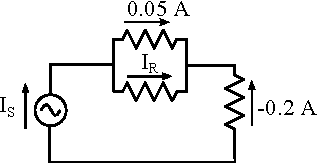
\includegraphics[width=0.7\textwidth]{kcl_oef.pdf}
		\caption{Vind $I_R$ en $I_s$.}
		\label{subfig:kcl_oef}
	\end{subfigure}
	~
	\begin{subfigure}[b]{0.45\linewidth}
		\centering
		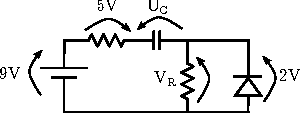
\includegraphics[width=0.9\textwidth]{kvl_oef.pdf}
		\caption{Vind $V_R$ en $U_C$. }
		\label{subfig:kvl_oef}
	\end{subfigure}
\caption{De wetten van Kirchhoff}
\label{fig:kirchoff_oef}
\end{figure}

Dit be�indigt de kennismaking met de elektronica. Je hebt nu alle basis die nodig is om aan de bouw van een versterker te beginnnen! Daar gaan we alleen nieuwe componenten leren kennen zoals de diode en de transistor, maar voor de rest is er niets nieuws onder de zon!

\section{Bouwstenen van de e-VUBOX}
\label{sec:bouwstenen}
In dit deel gaan we stap voor stap de onderdelen van onze versterker bouwen. We beginnen met een volumeregelaar, omdat we alles al kennen om die te maken. We gaan dan een simpele aan/uit LEDje ontwerpen zodat we weten wanneer onze versterker aan is. Daarna houden we ons bezig met de eigenlijke versterking en gaan we kennismaken met de transistor die ons daarmee gaat helpen. 

Maar eerst en vooral: waarom en hoe versterk je muziek?

\subsection{Versterken van audio}

Ook als je een student in elektronisch ingenieur bent, is een basiskennis in de rest van de wetenschappen toch handig. Want hoe versterk je geluid?

Geluid is een drukgolf door een lucht. De luchtdeeltjes bewegen heen en weer, en wanneer ze jouw trommelvlies raken, hoor je het geluid. Om het te versterken moeten we eerst de drukgolf omzetten naar een elektronengolf, die we gaan versterken, en dan terug naar een drukgolf zodat we het kunnen horen. Daarvoor gebruiken we twee componenten die je zowieso kent: de microfoon en de luidspreker.

% iets dat een elektronisch schakeling kan gebruiken. Daarvoor dient een microfoon! Het trillen van luchtdeeltjes wordt in een microfoon omgezet naar het trillen van elektronen. Voor de rest van het netwerk is de microfoon eigenlijk een spanningsbron.

%Een voorbeeld van een specifiek geluid is een muzieknoot. De muzieknoot ``la'' hoor je wanneer de luchtdruk op een zekere plaats golft met een frequentie\footnote{frequentie is het aantal volledige golven (op en neer) per seconde} van $440$ Hz. Je kan de luchtdrukgolf die we horen als een ``la'' wiskundig voorstellen als een sinus:

De microfoon vormt een drukgolf om naar een spanningsgolf. We kunnen een drukgolf uitdrukken als een sinus, met bijvoorbeeld een frequentie van $440$ Hz:
\begin{align}
	y(t) = A \cdot \sin (2\pi \cdot 440~\text{Hz} \cdot t)
\end{align}
met $y(t)$ de luchtdruk in Pascal, $A$ de amplitude van de drukgolf in Pascal en $t$ de tijd in seconden.

De microfoon gaat die drukgolf omvormen naar een spanningsgolf, met dezelfde frequentie (zie figuur \ref{fig:micro}.
\begin{figure}[htbp]
	\centering
	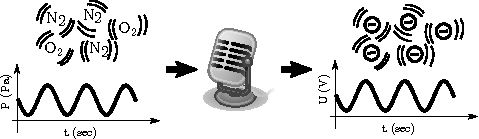
\includegraphics[width=0.95\textwidth]{micro}
	\caption{Een microfoon vormt de luchtdrukgolf (eenheid: Pascal) om in een spanningsgolf (eenheid: Volt).}
	\label{fig:micro}
\end{figure}

Om de muziek te kunnen horen moeten we de spanningsgolf terug omzetten naar een luchtdrukgolf, en daarvoor gebruiken we een luidspreker, die exact het omgekeerde doet van een microfoon. 

De luidspreker heeft wel ``sterkte'' nodig om luid muziek af te spelen. Om dat te doen moeten we het \textbf{elektrisch vermogen} over de luidspreker groot maken. Het elektrisch vermogen dat een component verbruikt wordt berekend als volgt:
\begin{align}
     P = V \cdot I
     \label{eq:vermogen}
 \end{align} 

 met $P$ het vermogen in Watt, $V$ het voltage over de component en $I$ de stroom door de component.

 Het doel van een versterker is dus om het vermogen van de muziek groter te maken! Nu dat we weten waarom ons netwerk nuttig is, kunnen we aan de bouw van onze versterker beginnen! Het ontwerpen van een versterker is, zoals je het zult zien, vooral het kiezen van veel weerstandswaarden.

\subsection{De volumeknop: de spanningsdeler}

We hebben de muziek dus omgevormd naar een spannings-signaal. Stel dat $V_s$ ons muzieksignaal is, en dat we in serie met die spanningsbron twee weerstanden schakelen (figuur \ref{fig:volume}), dan hebben we een zogenaamde \textbf{spanningsdeler} gebouwd. We gaan aantonen de spanning $V_2$ een verkleinde versie is van het muzieksignaal $V_s$. Dit is handig als het geluid te luid is, en dat we het volume willen regelen.

\begin{figure}[htbp]
	\centering
	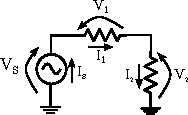
\includegraphics[width=0.3\textwidth]{weerstandsdeler}
	\caption{Volumeregeling: de spannignsdeler}
	\label{fig:volume}
\end{figure}

Om een netwerk op te lossen hebben we alleen de twee wetten van Kirchhoff nodig. In dit netwerk luiden ze:

\begin{align}
    I_S &= I_1 = I_2 \\
    V_S &- V_1 -V_2 = 0 
\end{align}

Samen met de wet van Ohm voor de twee weerstanden kunnen we alle stromen en spanningen bepalen.

\begin{align}
    V_1 = R_1 \cdot I_1 \\
    V_2 = R_2 \cdot I_2
\end{align}

\paragraph*{Doe-het-zelf:} Vind nu, dankzij de vier vorige vergelijkingen, de uitdrukking voor de spanning $V_2$ in functie van $V_s$, $R_1$ en $R_2$. Omdat we alleen de spanningsverhouding willen weten, mogen er geen stromen voorkomen in de formule.
\\.\dotfill \\.\dotfill \\.\dotfill \\.\dotfill \\
\begin{align}
    V_2 = \ldots\ldots
\end{align}
Je kan zien dat de spanning $V_2$, die we de uitgangsspanning noemen, altijd kleiner is dan (of gelijk aan) de ingangsspanning $V_s$. Daarom noemen we dit een spanningsdeler.
\paragraph*{Doe-het-zelf:} Je heb een voltage van $9$ V als ingangspanning $V_S$, en je wilt een voltage van $1.5$ V als uitgangspanning $V_2$. $R_1$ is al gekozen en heeft een weerstand van $1$ k$\Omega$ ($1000 \Omega$). Welke waarde moet je kiezen voor $R_2$?
\\.\dotfill \\.\dotfill \\.\dotfill \\.\dotfill \\
\begin{align}
    R_2 = \ldots\ldots
\end{align}
In de praktijk wordt een spanningdeler vaak met een regelbare weerstand gemaakt (zie figuur \ref{subfig:regelbareR}), zodat de verhouding tussen de in- en uitgangsspanning kan veranderd worden. In figuur \ref{subfig:pot} zie je een \textbf{potentiometer}, dat is een regelbare spanningsdeler. Het is eigenlijk een regelbare weerstand die je in het midden kan aftakken, en dat vormt een spanningsdeler omdat boven de aftakking een weerstand is, en eronder ook.

We gaan een potentiometer gebruiken als volumeknop! Omdat je een potentiometer volledig kunt toe- of opendraaien, maak de grootte van de weerstand niets uit voor de spannigsverhouding. Maar wat wel belangrijk is, is dat er niet te veel stroom door de potentiometer vloeit, want anders wordt er vermogen gebruikt door de volumeknop en gaan onze batterij zeer snel plat zijn. 

\paragraph*{Doe-het-zelf:} Welke weerstand $R$ moet de potentiometer hebben, wetend dat de ingangsspanning $V$ maximaal $200$ mV ( = $200 \cdot 10^{-3}$ V)is en we het vermogen $P$ willen beperken to 4 $\mu$W ( = $4 \cdot 10^{-6}$ W)? \textbf{Tip:} De formule voor elektrisch vermogen kan je vinden op pagina \pageref{eq:vermogen}, de je hebt de wet van Ohm ook nodig.
\\.\dotfill \\.\dotfill \\.\dotfill \\.\dotfill \\
\begin{align}
    R = \ldots\ldots
\end{align}

We hebben nu de waarde voor ��n component van onze versterker al gekozen. Laten we verder gaan met de aan/uit knop, zodat we snel naar de versterking kunnen gaan.
\begin{figure}
	\centering
	\begin{subfigure}[b]{0.45\linewidth}
		\centering
		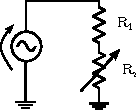
\includegraphics[width=0.5\textwidth]{regelbareR}
		\caption{Spanningsdeler met een regelbare weerstand (weerstand met een pijltje).}
		\label{subfig:regelbareR}
	\end{subfigure}
	~
	\begin{subfigure}[b]{0.45\linewidth}
		\centering
		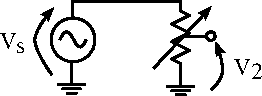
\includegraphics[width=0.8\textwidth]{potentiometer.pdf}
		\caption{Spanningsdeler met een potentiometer.}
		\label{subfig:pot}
	\end{subfigure}
\caption{Types spanningsdelers.}
\label{fig:vdeler} 
\end{figure}

\subsection{De aan/uit LED: de diode}
Een handig onderdeel op veel elektronische toestellen is het LED-lampje dat brandt om aan te geven dat het toestal aan is. LED staat voor Light Emitting Diode, dat we kunnen vertalen lichtgevende diode\footnote{Niet alle diodes zijn lichtegevend, diodes zijn ook van nut voor andere toepassingen.}. Een diode (figuur \ref{fig:diode}) is een heel belangrijke en nuttige elektronische component, die alleen stroom doorlaat in ��n richting.

\begin{figure}[htbp]
\centering
	\begin{subfigure}[b]{0.45\linewidth}
		\centering
		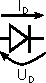
\includegraphics[width=0.2\textwidth]{diode}
		\caption{Een diode met voorwaarte spanning $U_D$ en stroom $I_D$. De diode laat alleen stroom toe in de  positieve stroomriching (richting van de stroompijl).}
		\label{fig:diode}
	\end{subfigure}
	~
	\begin{subfigure}[b]{0.45\linewidth}
		\centering
	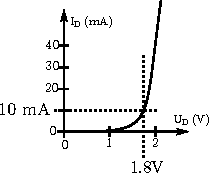
\includegraphics[width=0.8\textwidth]{diode_grafiek}
	\caption{Grafiek van de stroom in functie van de spanning van een diode.}
	\label{fig:diode_grafiek}
	\end{subfigure}
	\caption{Symbool en grafiek van een diode.}
\end{figure}

In figuur \ref{fig:diode_grafiek} zie je de grafiek van de stroom in functie van de spanning van de diode die we gaan gebruiken in onze versterker. In tegenstelling met de weerstand is de fysische wet van de diode niet-linear (= het is geen rechte), het is een exponenti�le functie. 

Omdat rekenen met een exponenti�le functie onhandig is, gaat een ingenieursstudent meestal eerst proberen om zich te redden met de grafiek. We gaan het circuit in figuur \ref{fig:diode_netwerk} oplossen zonder de die moeilijke functie te gebruiken.

\begin{figure}[htbp]
	\centering
	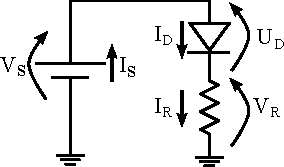
\includegraphics[width=0.3\textwidth]{diode_netwerk}
	\caption{Diode netwerk.}
	\label{fig:diode_netwerk}
\end{figure}

De keuze van de stroom door de LED bepaalt hoe fel het lichtje brand, dus die keuze gaan we als eerste maken. De datasheet\footnote{Een datasheet is een document dat de eigenschappen van elektronische componenten beschrijft.} stelt dat $10$ mA een typische stroomwaarde is voor onze LED. We zien dat op het grafiek in figuur \ref{fig:diode_grafiek} dat de voltage over de diode dan $1.8 $V moet zijn. De spanningsbron die we gaan gebruiken voor onze versterker is een 9V-batterij, dus $V_s = 9$ V. We zijn op zoek naar de weerstand die nodig is zodat de $U_D = 1.8$ V en $I_D =10$ mA. Om het netwerk op te lossen gebruiken we zoals altijd de wetten van Kirchhoff:
\begin{align}
	+V_s &- U_D - V_R = 0  \\
	I_s &= I_D = I_R
\end{align}
\paragraph*{Doe-het-zelf:} Kan je de waarde vinden van de weerstand die nodig is? \textbf{Tip:} bepaal $I_R$ en $V_R$ uit de wetten van Kirchhoff.
\\.\dotfill \\.\dotfill \\.\dotfill \\.\dotfill \\
\begin{align}
    R = \ldots\ldots
\end{align}

Om de aan/uit LED effectief te laten werken gaan we een schakelaar tussen de bron en de diode zetten zodat het licht alleen brandt wanneer het toestal aan is.

\subsection{De versterker: de transistor}
De transistor is een actieve elektronische component uitgevonden in $1947$, en is het baisingredi�nt van alle elektronische netwerken, van simpele versterkers tot een volledige PC. In tegenstelling met passieve componenten zoals de diode en de weerstand hebben actieve componenten nood aan een voeding, een externe energiebron die nodig is om ze te laten werken. Ze kunnen dankzij die extra energiebron (zoals een batterij) energie inpompen in een netwerk, en zijn dus handig voor versterking.

In figuur \ref{fig:sticky} vind je een kleine personage, Sticky, die verantwoordelijk is om een sluis te openen en te sluiten. Spijtig genoeg is Sticky niet de sterkste, en met een gewoon mechanisme zal het nooit lukken. Maar stel dat er een grote elektrische motor is die de tandwiel doet draaien, dan kan Sticky met ��n vinger de sluis openen en sluiten. De batterij en de motor doen eigenlijk al het werk voor Sticky.

Dit is eigenlijk hoe een transistor werkt! Met een zwak controlesignaal (Sticky), kan je een grote stroom controleren. Dit is heel vaak nuttig, omdat  signalen die komen uit optische sensoren, temperatuursensoren of micro's vaak heel zwak zijn.

 Een transistor kan als een schakelaar gebruikt worden: de stroom is dan ofwel helemaal  aan of helemaal uit. De tweede toepassing is de versterker: een kleine golf in het controlesignaal (Sticky maakt en golfje met de handvat van de motor) heeft een gigantische golf in de stroom als gevolg.

\begin{figure}[htbp]
\centering
	\begin{subfigure}[b]{0.45\linewidth}
		\centering
		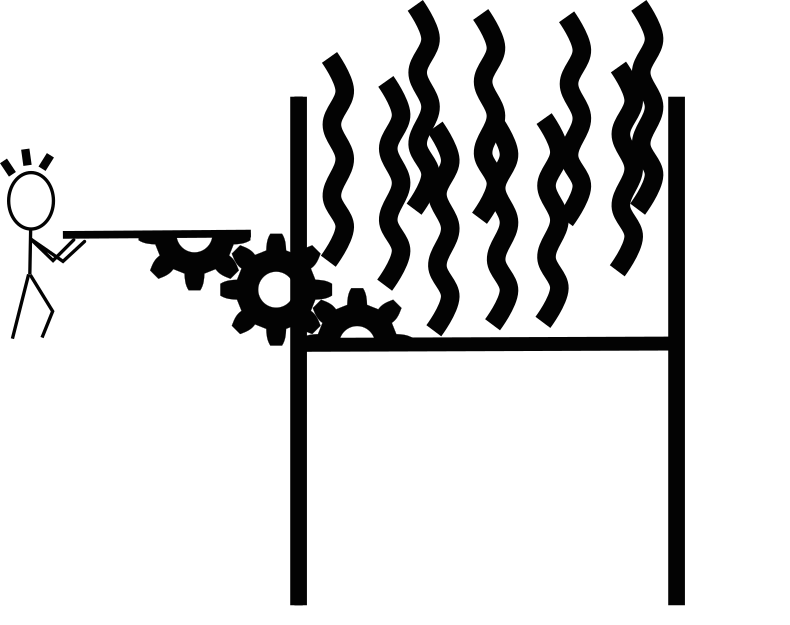
\includegraphics[width=\textwidth]{sitcky_closed}
		\caption{Sticky heeft het moeilijk om de sluis te openen.}
		\label{subfig:sticky_open}
	\end{subfigure}
	~
	\begin{subfigure}[b]{0.45\linewidth}
		\centering
	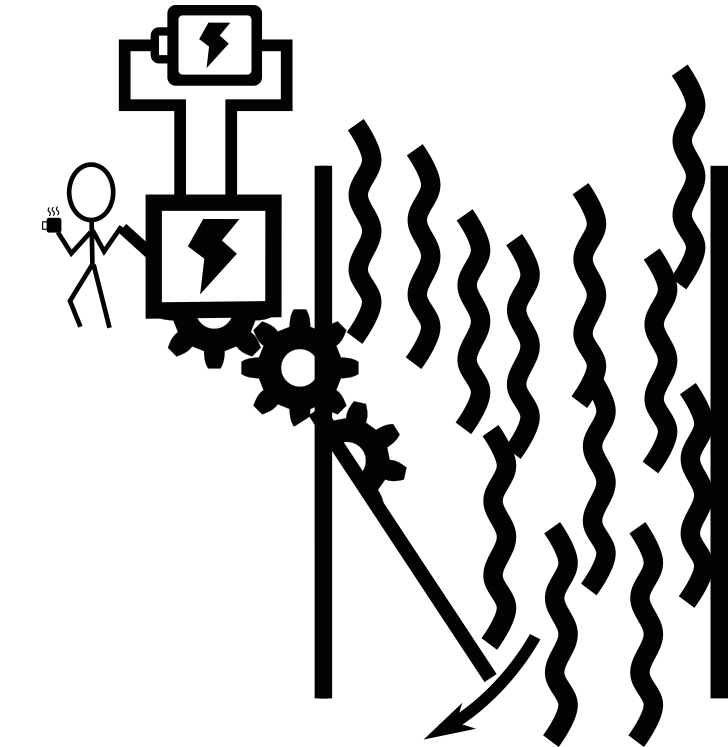
\includegraphics[width=0.85\textwidth]{sitcky_open}
	\caption{Dankzij de batterij moet Sticky bijna geen moeite doen om de sluis te bedienen.}
	\label{subfig:sticky_closed}
	\end{subfigure}
	\caption{Het verhaal van Sticky.}
	\label{fig:sticky}
\end{figure}

\subsubsection{De bipolaire npn transistor}
 Transistoren bestaan in verschillende types, wij gaan ons beperken tot de \emph{bipolaire NPN} transistor. Zoals je kan zien in figuur \ref{subfig:transistor_bce} is het een component met 3 pinnen, die elk een naam dragen: de basis, de collector en de emitter. De stroom $I_B$ (de basisstroom) is het controlesignaal die de rol opneemt van Sticky uit het verhaal hierboven.


\begin{figure}[htbp]
\centering
	\begin{subfigure}[b]{0.45\linewidth}
		\centering
		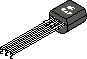
\includegraphics[width=0.25\textwidth]{transistor}
		\caption{De bipolaire transistor met Basis, Collector en Emitter aangeduid.}
		\label{subfig:transistor_bce}
	\end{subfigure}
	~
	\begin{subfigure}[b]{0.45\linewidth}
		\centering
	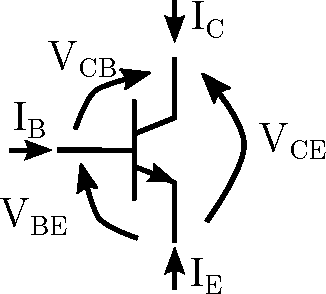
\includegraphics[width=0.7\textwidth]{transistor_VI}
	\caption{Bipolaire transistor met stromen en spanningen. Alle stromen worden conventioneel \textbf{naar} de transistor toe getekend.}
	\label{subfig:transistor_vi}
	\end{subfigure}
	\caption{De bipolaire npn transistor.}
	\label{fig:transistor}
\end{figure}

De fysische wetten die de relatie geeft tussen de stromen en de spanningen noemen de Ebers-Moll vergelijkingen. Zoals met de diode worden die niet vaak gebruikt tijdens het ontwerp, omdat ze te complex zijn. We kunnen dan  de grafieken gebruiken, maar voor de bipolaire transistor is er nog een derde weg: enkele regeltjes volstaan om te kunnen ontwerpen. 

De regels waaraan een bipolaire transistor zich moet houden zijn:
\begin{enumerate}
	\item De spanning op collector moet positiever zijn dan die op de basis: 
\begin{align}
    V_{CB} > 0~V. 
\end{align}
	\item De spanningsval tussen basis en emitter is ongeveer $0.7$ V: 
\begin{align}
    V_{BE} \approx 0.7~V
\end{align}

	\item $I_C, I_B$ en $V_{CE} $ moeten binnen bepaalde maximale waarden liggen, of de transistor gaat stuk (een transistor kan letterlijk in brand schieten, let op!).

	\item Als aan de drie vorige regels is voldaan, dan is de collectorstroom een versterkte versie van de basisstroom: 
	\begin{align}
	    I_C = \beta I_B
	    \label{eq:hfe}
	\end{align}
	$�\beta$ (ook als $h_{FE}$ genoteerd) wordt de stroomversterkingsfactor genoemd, en is typisch groter dan $50$, en kan soms $800$ gaan. Dit is waarom de nuttig is: een minuscuul kleine basisstroom controleert een veel grotere collectorstroom.

\end{enumerate}

De wetten van Kirchhoff gelden hier ook\footnote{We hebben hier eigenlijk de ``algemene'' wetten van Kirchoff gebruikt, waarvan de wetten van Kirchhoff die we hebben gezien zijn afgeleid. We kunnen inderdaad hier niet echt een knooppunt en een lus defin�ren in het ``midden'' van de transistor.}:

\begin{align}
    I_C		&+ I_B = -I_E \\
    V_{BE}  &+ V_{CB} - V_{CE} = 0
\end{align}

De stroomversterkingsfactor $\beta$ van een transistor is niet echt een te vertrouwen waarde: het kan afhangen van temperatuur, waar en wanneer het gemaakt werd, enz\ldots). We gaan dat getal niet in rekening brengen tijdens het ontwerp, omdat we alleen met zekerheid kunnen stellen dat het ``groot'' is. Maar dat is genoeg om een heel belangrijke conclusie te kunnen trekken...

\paragraph*{Doe-het-zelf:} Elimineer $I_B$ van de stroomwet van Kirchhoff met behulp van vergelijking (\ref{eq:hfe}). Vind dan een uitdrukking voor $I_C$. Stel dan dat $\beta = 250$, en rond af. Welke relatie vind je tussen $I_C$ en $I_E$? 
\\.\dotfill \\.\dotfill \\.\dotfill \\.\dotfill \\
\begin{align}
    I_C \approx \ldots \ldots
\end{align}

Een negative stroom is perfect mogelijk, dat wilt gewoon zeggen dat de stroom loopt tegen de pijlrichting in van figuur \ref{subfig:transistor_vi}. We zijn nu gereed om een versterkerschakeling op te lossen!

\subsubsection{De audio-versterker}
In figuur \ref{fig:ges} vind je een audio-versterker, waar je de bipolaire transistor in herkent. Je ziet dat we een actief netwerk hebben, er is een externe energiebron: de batterij $V_{CC}$. Je hebt dan de muziek de we gaan versterken in de spanningsbron $V_S$.

\begin{figure}[htbp]
	\centering
	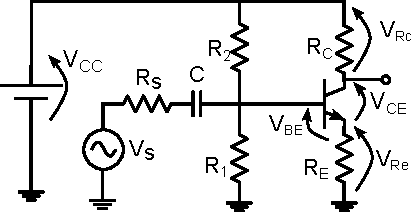
\includegraphics[width=0.8\textwidth]{ges}
	\caption{Versterkerschakeling met de transistor.}
	\label{fig:ges}
\end{figure}

In serie geschakeld met de spanningsbron $V_s$ is er een weerstand $R_s$ en een nieuwe component, de  capaciteit $C$. $R_s$ is de weerstand van de spanningsbron, die ons eigenlijk verveeld maar die in de werkelijkheid altijd aanwezig is. Het is de vaak klein genoeg dat ingenieursstudenten hem mogen verwaarlozen ( doen alsof $R_s = 0 \Omega$). 

De capaciteit is een component die voldoet aan de wet : 
\begin{align}
    I = C \cdot \frac{dV}{dt}
\end{align}

Dat betekent ruwweg dat capaciteiten alleen reageren op \emph{verandering in de spanning}, en niet op constante waarden. Zonder het te bewijzen kunnen we verklappen dat het gevolg van die capaciteit is dat de spanning in het knooppunt\footnote{Herinner U: Als we spreken van een spanning in een punt, bedoelen we eigenlijk de spanningsval tussen dat punt en de grond.} 1 de som gaat zijn van $V_s$ en van de spanning omwille van de weerstandsdeler $R_1,R_2$ en $V_{CC}$:
\begin{align}
    V_{B} = V_s + \frac{R_1}{R_1+R_2}V_{CC}
\end{align}

Om de versterker te ontwerpen moeten we de weerstanden $R_1,R_2,R_E$ en $R_C$ kiezen. Een eerste vergelijking die belangrijk gaan we nu afleiden: de spanningsversterking van dit netwerk.

\paragraph*{Doe-het-zelf:} Vind een uitdrukking voor de spanning aan de collector $V_C$ in functie van de basisspanning $V_B$, en vind dat je de spanning $V_B$ versterkt. We hebben volgende vergelijkingen die we kunnen gebruiken:
\begin{itemize}
	\item de spanningswet van Kirchoff
	\begin{align}
	V_{Re} + V_{CE} + V_{Rc} - V_{CC} = 0    
	\end{align}
	\item de transistorvergelijkingen
	\begin{align}
    V_{BE} &= V_{B} - V_{E} = 0.7~V \\
     I_C&\approx -I_E \\
    V_{CE} &= V_C - V_E > 0
	\end{align}
	\item de weerstandsvergelijkingen
	\begin{align}
   	V_{Rc} &= R_C \cdot I_C \\
   	V_{Re} &= - R_E \cdot  I_E
	\end{align}
	De wet van Ohm geldt als de spanning- en stroomrichting tegengesteld zijn. Indien ze in dezelfde richting zijn, komt er een minteken in de wet.
\end{itemize}

\textbf{Tip:} ��n manier om het te vinden: druk de stroom uit door $R_C$ met de wet van Ohm. Die is nodig om de spanning $V_E$ te vinden die je dan gebruikt om $V_B$ te vinden. Vorm de vergelijking dan om om $V_C$ te isoleren.
\\.\dotfill \\.\dotfill \\.\dotfill \\.\dotfill \\.\dotfill \\.\dotfill \\.\dotfill \\.\dotfill 

\begin{align}
    V_C = \ldots \ldots \ldots \ldots  \ldots  \ldots 
\end{align}

We kunnen de constante (DC) termen eventjes vergeten en drukken alleen de tijdsvari�rende (AC) spanning gedeelte uit van $V_C$, die we met kleine letters noteren:

\begin{align}
    v_c = - \frac{R_C}{R_E} \cdot v_b
\end{align}

Deze schakeling versterkt dus de spanningsgolf met een factor $- \frac{R_C}{R_E}$, de muziekgolf wordt dus omgedraaid en de amplitude versterkt! De andere DC waarde wilt alleen zeggen dat het gemiddelde van de golf zich verplaatst, zoals je kan zien in figuur \ref{fig:golven}.

\begin{figure}[htbp]
	\centering
	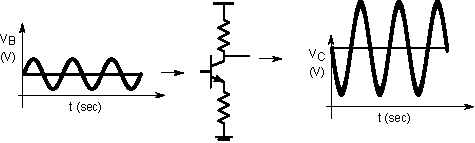
\includegraphics[width=0.95\textwidth]{golven}
	\caption{De ingangsgolf wordt door ons netwerk omgedraaid en versterkt, en het gemiddelde verschuift.}
	\label{fig:golven}
\end{figure}

We gaan nu een ontwerpmethodevolgen waar verschillende keuzes moeten gemaakt worden, waaruit de waardes voor de weerstanden uit volgen. Eens je de methode kent, kan je andere keuzes proberen maken en zien als het werkt: dit is wat ontwerpen is! Niet alle designers gaan het graag zeggen, maar een groot deel van ontwerp is vallen en opstaan: uitproberen tot dat het werkt. En daar is niets mis mee (als je maar niets opblaast)!

De methode gaat als volgt:
\begin{enumerate}
	\item Kies de typische stroom $I_C$. De maximumwaarde die de transistor aankan is $100~mA$, dus het moet kleiner. Te grote stromen gaan ook de batterij sneller leegzuigen, te kleine stromen kunnen de werking van het netwerk stopzetten. Er zijn nog  andere voor- en nadelen die je kan uitzoeken voor te grote of te kleine stromen. We kiezen als voorbeeld:
\begin{align}
    I_C = 10 mA
\end{align}

	\item Kies een typisch voltage $V_C$, waar de muziekgolf rond gaat vari�ren. Dit noemen we het instelpunt. De spanning $V_C$ moet groter zijn dan $0.7~V$ (dat kan je afleiden uit de spanningswet van Kirchhoff en  $V_{CB} > 0$, en $V_{BE} = 0.7$). De transistor kan hier de spanning aan zijn pinnen niet hoger krijgen dan zijn voeding. De maximum is dus $V_{CC} = 9~V$. Pas op, een batterij gaat slijten, na een tijdje kan de geleverde spanning zo laag als $7~V$ gaan. De voorbeeldkeuze die wie hier maken is:

\begin{align}
    V_C =  3.5~V
\end{align}
	 Dat is ongeveer in het midden tussen $7~V$ en $0.7~V$. Je kan snappen waarom het midden een mogelijke keuze is door een tekening te maken zoals in figuur \ref{fig:golven}. Dit is niet de enige mogelijkheid!

	\item Laatste keuze: kies een versterkingsfactor $- \frac{R_C}{R_E}$. Als je de amplitude van de inkomende golf $V_S$ kent, dan kan de versterkingsfactor zo kiezen dat je uitgaande spanningsgolf zeker niet boven $V_{CC}$ komt, of onder $0$ V (=de grond). Spijtig genoeg is er geen standaardwaarde voor de amplitude van een muzieksignaal, maar het is meestal klein en ongeveer  $200~mV$. We kunnen bijvoorbeeld zeggen dat we de amplitude naar $1V$ willen krijgen, we hebben dus een versterkingsfactor nodig van $-5$.
	\begin{align}
	    \frac{R_C}{R_E} = 5
	\end{align}
\end{enumerate}

Vergeet zeker niet dat dit niet vaste keuzes zijn, er zijn veel andere mogelijkheden, probeer vast en zeker te spelen met andere waardes!

\paragraph*{Doe-het-zelf:} Je kent nu alles wat nodig is om de weerstanden $R_{E}$ en $ R_{C}$ te bepalen. \textbf{Tip:} Uit $I_C$ en $V_C$ kan je de waarde $R_C$ vinden.
\\.\dotfill \\.\dotfill \\.\dotfill \\.\dotfill \\.\dotfill \\.\dotfill \\.\dotfill \\.\dotfill 
\begin{align}
    R_C &= \ldots \\
    R_E &= \ldots
\end{align}

De vaste waarde waarond $V_B$ gaat vari�ren ligt nu al vast (omdat $V_{BE} = 0.7V$), en noemen we het biaspunt. We kunnen die vastleggen met de weerstandsdeler $R_1$ en $R_2$. Alhoewel het geen zuivere weerstandsdeler is (normaal gezien is niets aangesloten aan een weerstandseler), kunnen toch de formule van de weerstandsdeler gebruiken hier.

\paragraph*{Doe-het-zelf:} Bereken het biasvoltage $V_B$. Kies dan de weerstand $R_2$ zodat $V_B$ de gewenste waarde heeft. Het staat al vast dat $R_1 = 1k\Omega$. \textbf{Tip:} Herinner U dat $V_{CC} = 9V$ en de formule van de weerstandsdeler.
\\.\dotfill \\.\dotfill \\.\dotfill \\.\dotfill \\.\dotfill \\.\dotfill \\.\dotfill \\.\dotfill \\.\dotfill \\.\dotfill \\.\dotfill \\.\dotfill \\.\dotfill \\.\dotfill \\.\dotfill \\.\dotfill 

\begin{align}
    R_1 &= 1k\Omega \\
    R_2 &= \ldots
\end{align}

En voor dat je het weet, hebben we de versterker helemaal gemaakt! Je kan zien dat we vermogen hebben versterkt van het ingangssignaal:

\begin{enumerate}
 	\item de amplitude van de stroom $I_B$ is enkele $\mu$A, terwijl de amplitude van $I_C$ enkele mA bedraagt
 	\item de amplitude van de spanning $V_B$ is enkele mV, terwijl de amplitude van $V_E$ in de grootteorde van  1 Volt is.
 \end{enumerate} 

 De stroom en de spanning zijn  versterkt, dus het vermogen is gestegen! We zijn vertrokken van enkele $\mu$W en we hebben nu uiteindelijk enkele $m$W. 

\begin{center}
	\noindent \fbox{ 
    \parbox{0.8\textwidth}{
Samenvatting van de gekozen weerstanden:
\begin{align}
    R_1 &= \ldots \\
    R_2 &= \ldots \\
    R_E &= \ldots \\
    R_C &= \ldots
\end{align}
    }}
\end{center}

\subsection{De magische zwarte doos}

\subsection{De luidspreker}

\section{Conclusie}

\section{Nagerecht}
\subsection{De hoogdoorlaatfilter en de capaciteit.}
\subsection{Hoe lang gaat de versterker mee?}

\end{document}